\section{Thiết kế kiến trúc tổng
thể}

Hệ thống được thiết kế theo kiến trúc phân tầng. Tầng giao diện tiếp
nhận thao tác của người dùng và quản trị viên; tầng backend xử lý xác
thực, định tuyến API, quản trị dữ liệu và điều phối pipeline RAG; tầng
AI/RAG thực hiện chuẩn hóa truy vấn, truy xuất ngữ nghĩa, rerank và sinh
câu trả lời; tầng lưu trữ gồm Firestore cho dữ liệu nghiệp vụ và
ChromaDB cho vector tri thức. Cách chia này giúp khóa dịch vụ, service
account và logic AI không bị đưa ra phía trình duyệt.

Trong mã nguồn, backend FastAPI được chia thành ba router chính: auth,
user và admin. Router auth xử lý token Firebase, kiểm tra quyền admin,
gửi OTP và xác minh OTP. Router user xử lý chat, session và lịch sử hội
thoại. Router admin xử lý thống kê, người dùng, tài liệu, backup, quản
lý admin, chuyển văn bản sang JSON và reload vector database. Các module
RAG như pipeline, chunker, intent, normalizer, memory và vectorstore
được tách riêng để dễ kiểm thử và thay đổi.

\begin{itemize}
\item
  Frontend: React, TypeScript, Vite và Tailwind CSS; gồm ChatBox,
  Sidebar, LoginPage, InputBox, Message và AdminDashboard.
\item
  Backend: FastAPI; chia nhóm API thành auth, user và admin; kiểm tra
  Firebase ID Token trước khi xử lý các chức năng cần bảo vệ.
\item
  AI/RAG: xử lý intent, rewrite câu hỏi theo lịch sử, chuẩn hóa synonym,
  semantic retrieval, CrossEncoder rerank, prompt ràng buộc và LLM
  fallback.
\item
  Lưu trữ: Firestore lưu session, message, OTP và settings; ChromaDB lưu
  embedding và metadata của các chunk thủ tục.
\end{itemize}

\begin{figure}[H]
\centering
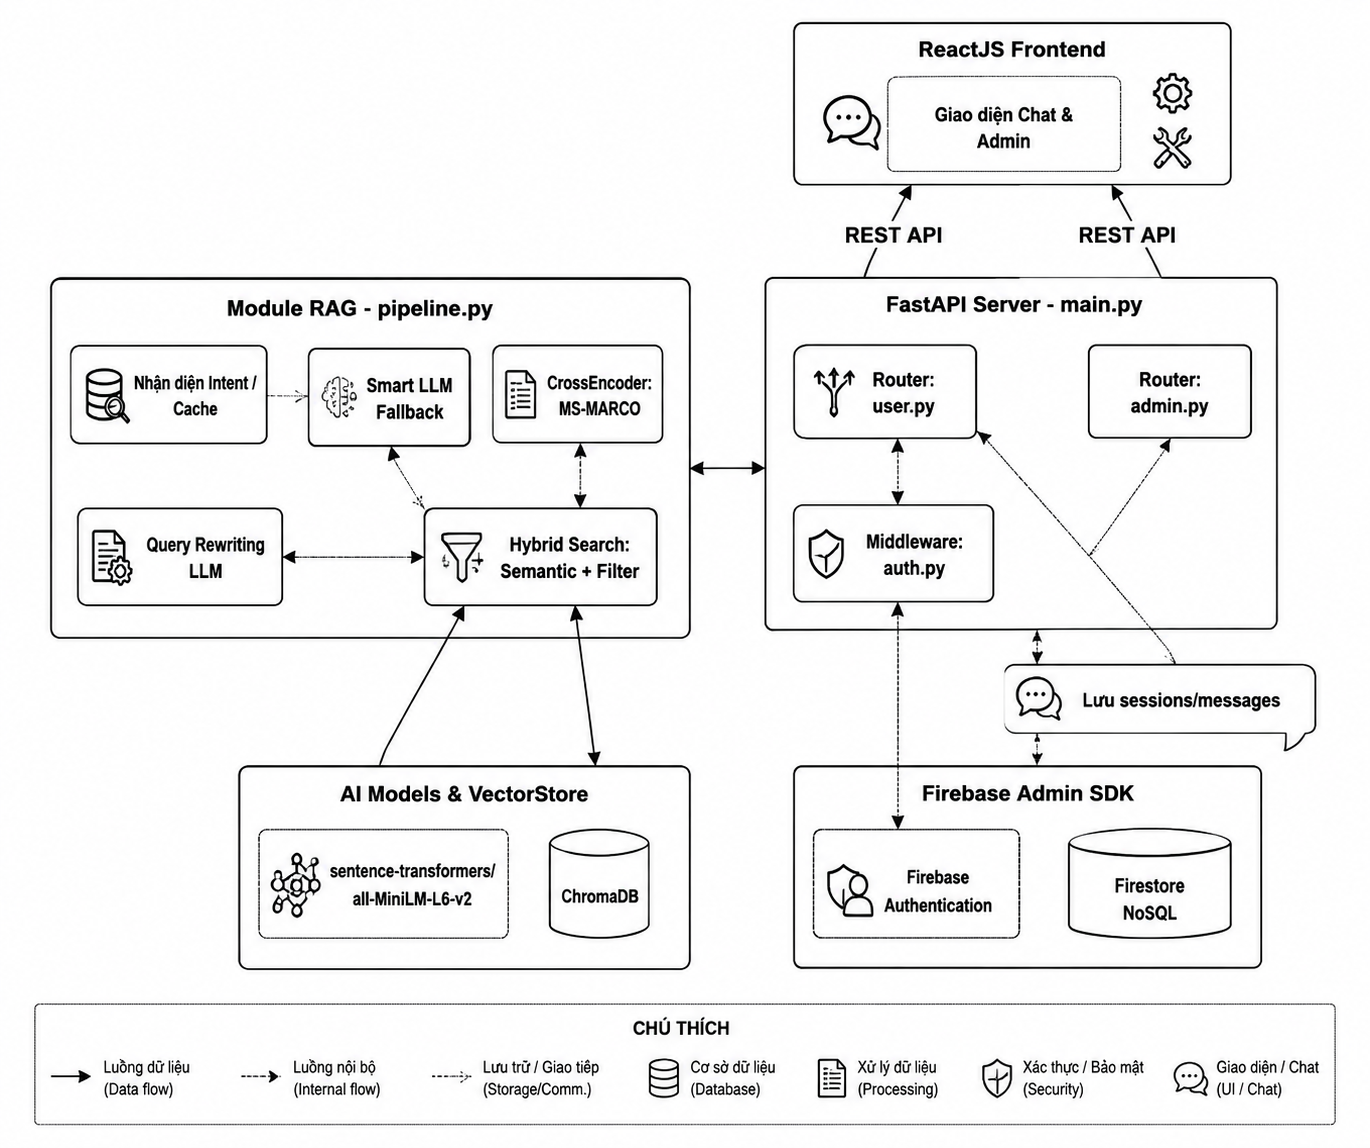
\includegraphics[width=0.92\textwidth]{tai_nguyen/media/image7.png}
\caption{Kiến trúc tổng thể của hệ thống chatbot RAG}
\label{fig:3-1}
\end{figure}

\section{Thiết kế mô hình lớp thực thể và
quan
hệ}

Để đáp ứng yêu cầu về Entity Class Diagram, hệ thống được mô hình hóa ở
mức thực thể nghiệp vụ thay vì chỉ trình bày bảng collection Firestore.
Các thực thể chính gồm User, Admin, Session, Message, Procedure,
ProcedureChunk, OTPCode, AdminSetting, BackupSetting và BackupRecord. Mô
hình này phản ánh cả dữ liệu người dùng, dữ liệu hội thoại, dữ liệu thủ
tục và dữ liệu vận hành vector database.

\begin{figure}[H]
\centering
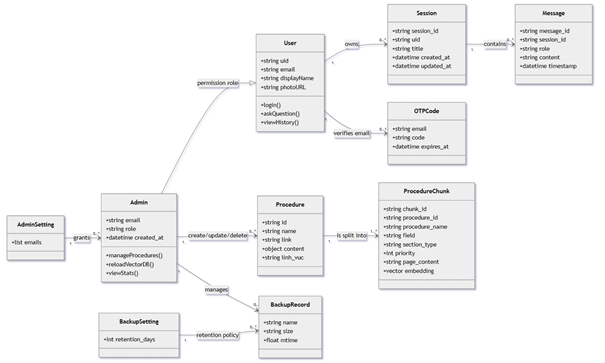
\includegraphics[width=0.92\textwidth]{tai_nguyen/media/image8.png}
\caption{Entity Class Diagram của hệ thống}
\label{fig:3-2}
\end{figure}

Quan hệ dữ liệu cốt lõi của hệ thống có thể hiểu như sau: một User có
nhiều Session; một Session có nhiều Message; một Procedure được chia
thành nhiều ProcedureChunk; Admin là người dùng có quyền đặc biệt để
quản lý Procedure và BackupRecord. ChromaDB không phải cơ sở dữ liệu
quan hệ, nhưng về thiết kế logic, mỗi chunk vẫn cần gắn với một thủ tục
thông qua procedure\_id để phục vụ truy xuất và trích dẫn nguồn.

\begin{figure}[H]
\centering
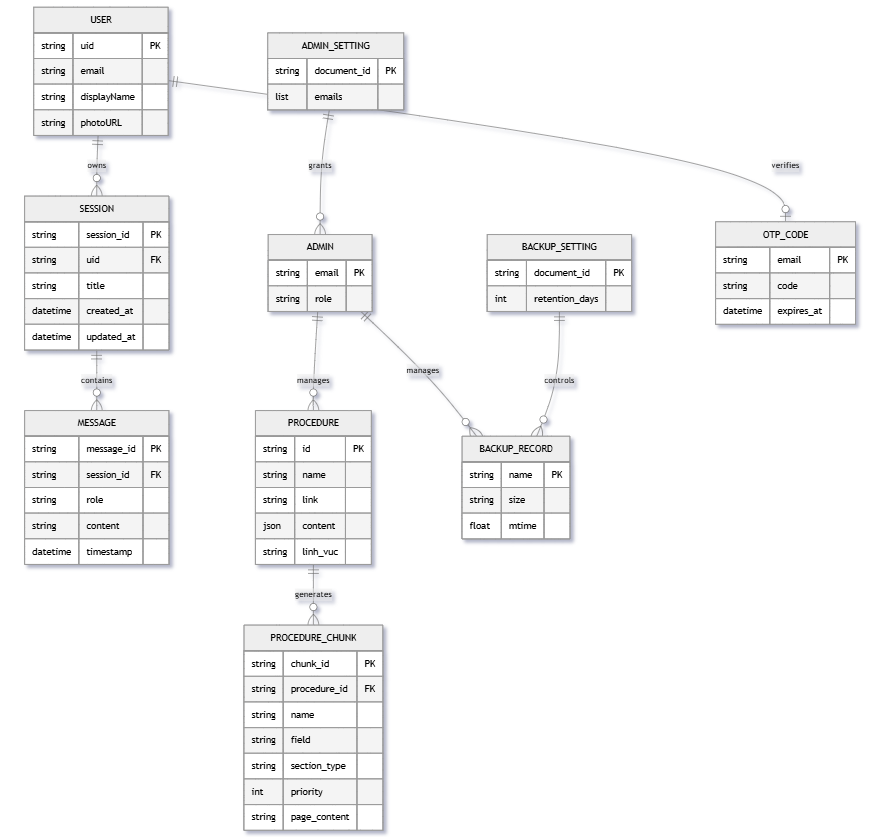
\includegraphics[width=0.92\textwidth]{tai_nguyen/media/image9.png}
\caption{Sơ đồ quan hệ dữ liệu User - Session - Message - Procedure - Chunk - Admin}
\label{fig:3-3}
\end{figure}

\begin{longtable}[]{|
  >{\raggedright\arraybackslash}p{(\columnwidth - 4\tabcolsep) * \real{0.2167}}|
  >{\raggedright\arraybackslash}p{(\columnwidth - 4\tabcolsep) * \real{0.3827}}|
  >{\raggedright\arraybackslash}p{(\columnwidth - 4\tabcolsep) * \real{0.4006}}|}
\caption{Thiết kế lớp thực thể chính}\\
\hline
\begin{minipage}[b]{\linewidth}\raggedright
\textbf{Lớp thực thể}
\end{minipage} & \begin{minipage}[b]{\linewidth}\raggedright
\textbf{Thuộc tính tiêu biểu}
\end{minipage} & \begin{minipage}[b]{\linewidth}\raggedright
\textbf{Vai trò}
\end{minipage} \\
\hline
\endfirsthead
\continuedcaption{Thiết kế lớp thực thể chính}
\hline
\begin{minipage}[b]{\linewidth}\raggedright
\textbf{Lớp thực thể}
\end{minipage} & \begin{minipage}[b]{\linewidth}\raggedright
\textbf{Thuộc tính tiêu biểu}
\end{minipage} & \begin{minipage}[b]{\linewidth}\raggedright
\textbf{Vai trò}
\end{minipage} \\
\hline
\endhead
\hline
\endlastfoot
User & uid, email, displayName, photoURL & Đại diện người dùng đã xác
thực qua Firebase. \\
\hline
Admin & email, role, created\_at & Người dùng có quyền truy cập
dashboard và API quản trị. \\
\hline
Session & session\_id, uid, title, created\_at, updated\_at & Phiên hội
thoại giữa người dùng và chatbot. \\
\hline
Message & message\_id, session\_id, role, content, timestamp & Tin nhắn
trong một phiên; role có thể là user hoặc bot. \\
\hline
Procedure & id, name, link, content, linh\_vuc & Thủ tục hành chính
trong procedures.json. \\
\hline
ProcedureChunk & chunk\_id, procedure\_id, field, section\_type,
priority, page\_content & Đoạn tri thức đã được chia nhỏ và lưu trong
ChromaDB. \\
\hline
OTPCode & email, code, expires\_at & Mã xác minh tạm thời khi đăng ký
tài khoản email. \\
\hline
BackupRecord & name, size, mtime & Bản sao lưu ChromaDB tạo trước khi
reload. \\
\hline
\end{longtable}

\section{Thiết kế cơ sở dữ
liệu}

Firestore và ChromaDB được sử dụng song song vì hai nhóm dữ liệu có bản
chất khác nhau. Firestore phù hợp với dữ liệu nghiệp vụ có định danh,
thời gian và quan hệ theo người dùng. ChromaDB phù hợp với dữ liệu văn
bản đã được nhúng thành vector để phục vụ tìm kiếm ngữ nghĩa. Thiết kế
này giúp hệ thống vừa quản lý được lịch sử hội thoại, vừa truy xuất được
dữ liệu thủ tục theo ý nghĩa câu hỏi.

Trong mã nguồn, lịch sử hội thoại được lưu theo collection sessions và
sub-collection messages. Hàm save\_message tạo hoặc cập nhật document
session, sau đó thêm từng tin nhắn vào sub-collection messages với role,
content và timestamp. Hàm get\_history chỉ lấy một số tin nhắn gần nhất
để đưa vào prompt, tránh làm prompt quá dài và giảm rủi ro đưa dư dữ
liệu cá nhân vào LLM.

\begin{longtable}[]{|
  >{\raggedright\arraybackslash}p{(\columnwidth - 4\tabcolsep) * \real{0.2921}}|
  >{\raggedright\arraybackslash}p{(\columnwidth - 4\tabcolsep) * \real{0.2929}}|
  >{\raggedright\arraybackslash}p{(\columnwidth - 4\tabcolsep) * \real{0.4150}}|}
\caption{Thiết kế các collection chính trên Firestore}\\
\hline
\begin{minipage}[b]{\linewidth}\raggedright
\textbf{Collection}
\end{minipage} & \begin{minipage}[b]{\linewidth}\raggedright
\textbf{Trường chính}
\end{minipage} & \begin{minipage}[b]{\linewidth}\raggedright
\textbf{Mục đích}
\end{minipage} \\
\hline
\endfirsthead
\continuedcaption{Thiết kế các collection chính trên Firestore}
\hline
\begin{minipage}[b]{\linewidth}\raggedright
\textbf{Collection}
\end{minipage} & \begin{minipage}[b]{\linewidth}\raggedright
\textbf{Trường chính}
\end{minipage} & \begin{minipage}[b]{\linewidth}\raggedright
\textbf{Mục đích}
\end{minipage} \\
\hline
\endhead
\hline
\endlastfoot
sessions & uid, title, created\_at, updated\_at & Lưu thông tin phiên
hội thoại. \\
\hline
sessions/\{id\}/messages & role, content, timestamp & Lưu từng tin nhắn
trong một phiên chat. \\
\hline
otp\_codes & code, expires\_at & Lưu OTP tạm thời, hết hạn sau 5
phút. \\
\hline
settings/admins & emails & Lưu danh sách email có quyền quản trị. \\
\hline
settings/backup & retention\_days & Lưu số ngày giữ backup ChromaDB. \\
\hline
\end{longtable}

Đối với ChromaDB, mỗi chunk lưu page\_content và metadata. Metadata được
tạo từ chunker.py, trong đó có procedure\_id, name, field,
section\_type, priority và chunk\_id. Các chunk được tạo theo nhóm tổng
quan, cách thức thực hiện, thành phần hồ sơ, căn cứ pháp lý và các
trường đơn giản. Với phí và lệ phí, chunker xử lý liên kết phí theo từng
hình thức thực hiện để tránh mất ngữ cảnh.

\begin{longtable}[]{|
  >{\raggedright\arraybackslash}p{(\columnwidth - 4\tabcolsep) * \real{0.2433}}|
  >{\raggedright\arraybackslash}p{(\columnwidth - 4\tabcolsep) * \real{0.2492}}|
  >{\raggedright\arraybackslash}p{(\columnwidth - 4\tabcolsep) * \real{0.5075}}|}
\caption{Thiết kế metadata cho dữ liệu trong ChromaDB}\\
\hline
\begin{minipage}[b]{\linewidth}\raggedright
\textbf{Trường metadata}
\end{minipage} & \begin{minipage}[b]{\linewidth}\raggedright
\textbf{Ý nghĩa}
\end{minipage} & \begin{minipage}[b]{\linewidth}\raggedright
\textbf{Ví dụ}
\end{minipage} \\
\hline
\endfirsthead
\continuedcaption{Thiết kế metadata cho dữ liệu trong ChromaDB}
\hline
\begin{minipage}[b]{\linewidth}\raggedright
\textbf{Trường metadata}
\end{minipage} & \begin{minipage}[b]{\linewidth}\raggedright
\textbf{Ý nghĩa}
\end{minipage} & \begin{minipage}[b]{\linewidth}\raggedright
\textbf{Ví dụ}
\end{minipage} \\
\hline
\endhead
\hline
\endlastfoot
procedure\_id / id & Mã thủ tục hành chính. & 2.002307.000.00.00.H35 \\
\hline
name / procedure\_name & Tên thủ tục. & Giải quyết chế độ mai táng phí
đối với cựu chiến binh \\
\hline
linh\_vuc & Lĩnh vực quản lý. & Người có công \\
\hline
field & Trường dữ liệu gốc. & Thành phần hồ sơ \\
\hline
section\_type & Loại chunk ngữ nghĩa. & summary, method, document,
legal, simple \\
\hline
chunk\_id & Định danh chunk. & 2.002307.000.00.00.H35\_document\_1 \\
\hline
priority & Mức ưu tiên khi truy xuất. & 10 \\
\hline
\end{longtable}

\section{Thiết kế pipeline RAG và trích dẫn
nguồn}

\begin{figure}[H]
\centering
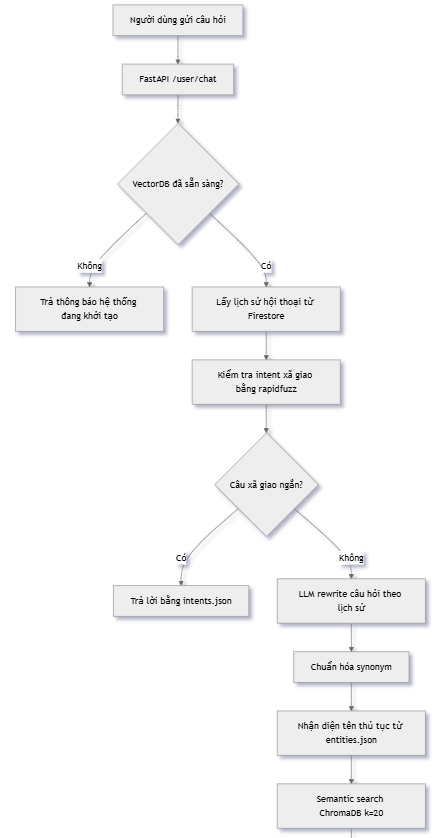
\includegraphics[height=0.74\textheight,keepaspectratio]{tai_nguyen/media/image10.png}
\caption{Luồng xử lý câu hỏi bằng pipeline RAG (a)}
\label{fig:3-4}
\end{figure}
Pipeline
RAG gồm hai pha: nạp dữ liệu và hỏi đáp. Pha nạp dữ liệu đọc
procedures.json, làm sạch văn bản, chia semantic chunks, gắn metadata,
sinh embedding và lưu vào ChromaDB. Pha hỏi đáp nhận câu hỏi của người
dùng, lấy lịch sử gần nhất, xử lý intent, rewrite câu hỏi nếu cần, chuẩn
hóa synonym, truy xuất ChromaDB, rerank bằng CrossEncoder, chọn context
và gọi LLM để sinh câu trả lời.

Trong code hiện tại, endpoint chat gọi ask\_rag với db, query,
session\_id và history. Bên trong pipeline, câu hỏi ngắn thuộc nhóm xã
giao được handle\_intent xử lý sớm. Nếu là câu nghiệp vụ, hệ thống có
thể dùng LLM nhẹ để rewrite câu hỏi dựa trên lịch sử, sau đó
normalize\_query, detect\_procedure\_name và detect\_field. Retrieval
gồm semantic search k=20 và truy xuất bổ sung có filter theo tên thủ tục
k=10 nếu nhận diện được thủ tục. Các tài liệu được loại trùng, rerank
bằng CrossEncoder và chọn tối đa 10 chunk làm context.

\begin{figure}[H]
\centering
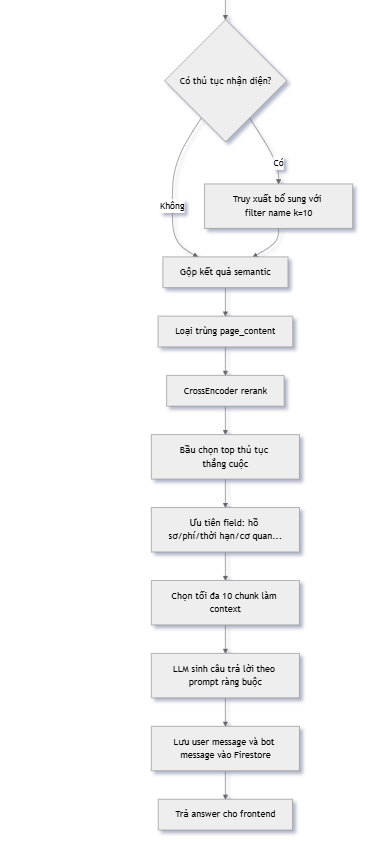
\includegraphics[height=0.74\textheight,keepaspectratio]{tai_nguyen/media/image11.png}
\caption{Luồng xử lý câu hỏi bằng pipeline RAG (b)}
\label{fig:3-5}
\end{figure}
Để
khắc phục hạn chế về việc chưa hiển thị nguồn chi tiết cho từng câu trả
lời, hệ thống có thể được mở rộng thêm cơ chế trích dẫn nguồn. Theo
thiết kế đề xuất, kết quả trả về của pipeline RAG không chỉ gồm nội dung
trả lời mà còn kèm danh sách nguồn dữ liệu đã được sử dụng trong quá
trình sinh câu trả lời.

Danh sách nguồn có thể được lấy từ metadata của các chunk sau bước truy
xuất, rerank và lọc theo trường thông tin. Mỗi nguồn gồm các thông tin
như mã thủ tục, tên thủ tục, mục dữ liệu được sử dụng, mã chunk và đường
dẫn trang nguồn nếu dữ liệu gốc có cung cấp. Khi hiển thị trên giao
diện, frontend có thể đặt phần ``Nguồn tham khảo'' ở cuối câu trả lời để
người dùng kiểm chứng lại thông tin.

Cách thiết kế này giúp tăng tính minh bạch của chatbot hành chính công.
Người dân có thể biết câu trả lời được tổng hợp từ thủ tục nào, còn quản
trị viên có thêm căn cứ để kiểm tra khi hệ thống truy xuất nhầm chunk
hoặc dữ liệu nguồn chưa được chuẩn hóa tốt.

\begin{figure}[H]
\centering
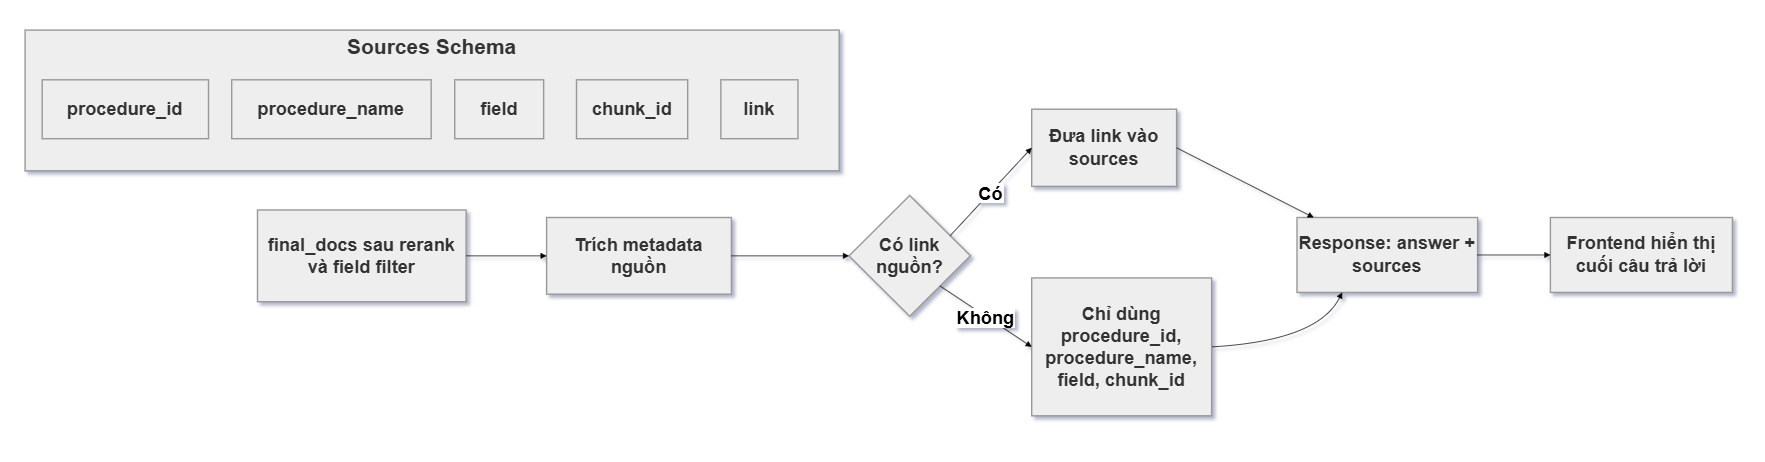
\includegraphics[width=0.92\textwidth]{tai_nguyen/media/image12.png}
\caption{Thiết kế trích dẫn nguồn trong câu trả lời}
\label{fig:3-6}
\end{figure}

\begin{longtable}{|>{\raggedright\arraybackslash}p{0.27\textwidth}|>{\raggedright\arraybackslash}p{0.35\textwidth}|>{\raggedright\arraybackslash}p{0.30\textwidth}|}
\caption{Thiết kế nguồn trích dẫn trong câu trả lời}\\
\hline
\textbf{Trường} & \textbf{Mô tả} & \textbf{Ví dụ} \\
\hline
\endfirsthead
\continuedcaption{Thiết kế nguồn trích dẫn trong câu trả lời}
\hline
\textbf{Trường} & \textbf{Mô tả} & \textbf{Ví dụ} \\
\hline
\endhead
\hline
\endlastfoot
\codepathraw{answer} & Câu trả lời cuối cùng của chatbot. & Hồ sơ gồm... \\
\hline
\codepath{sources[].procedure_id} & Mã thủ tục dùng làm nguồn. & \codepathraw{2.002307.000.00.00.H35} \\
\hline
\codepath{sources[].procedure_name} & Tên thủ tục dùng làm nguồn. & Giải quyết chế độ mai táng phí đối với cựu chiến binh \\
\hline
\codepath{sources[].field} & Mục thông tin được sử dụng. & Thành phần hồ sơ \\
\hline
\codepath{sources[].chunk_id} & Chunk cụ thể trong ChromaDB. & \codepathraw{2.002307.000.00.00.H35_document_1} \\
\hline
\codepath{sources[].link} & Đường dẫn trang nguồn nếu có. & URL trang chi tiết thủ tục \\
\hline
\end{longtable}

\section{Thiết kế API và request/response
mẫu}

API của hệ thống được chia thành ba nhóm chính: auth, user và admin.
Nhóm auth phục vụ xác thực người dùng, gửi OTP và kiểm tra quyền quản
trị; nhóm user phục vụ các chức năng phía người dân như hỏi đáp chatbot,
lấy danh sách phiên và xem lịch sử hội thoại; nhóm admin phục vụ thống
kê, quản lý dữ liệu thủ tục, chuyển văn bản sang JSON, quản lý backup và
đồng bộ lại vector database. Cách tách nhóm API này giúp backend kiểm
soát quyền truy cập rõ ràng, đồng thời giúp frontend gọi đúng nhóm chức
năng theo vai trò người dùng.

Trong mã nguồn hiện tại, endpoint /user/chat đang được cài đặt bằng
phương thức GET với tham số q và session\_id. Endpoint này kiểm tra
token Firebase, lấy lịch sử hội thoại, gọi pipeline RAG, sau đó lưu tin
nhắn của người dùng và câu trả lời của bot vào Firestore bằng background
task. Tuy nhiên, nếu xét theo thiết kế REST hoàn thiện, nghiệp vụ gửi
câu hỏi nên chuyển sang POST vì request có nội dung nghiệp vụ, cần xác
thực, có thể truyền body JSON và phát sinh tác động ghi lịch sử hội
thoại. Do đó, phần thiết kế dưới đây ghi rõ cả hiện trạng mã nguồn và
phương án đề xuất để thuận lợi khi nâng cấp.

Ngoài API hỏi đáp chatbot, hệ thống nên bổ sung thêm hai API phía người
dùng để bám đầy đủ Use Case tra cứu thủ tục và xem chi tiết thông tin
thủ tục. Trong phiên bản hiện tại, người dùng chủ yếu tra cứu qua
chatbot RAG; dữ liệu thủ tục đầy đủ đang được quản lý ở phía admin thông
qua /admin/documents. Khi hoàn thiện sản phẩm, có thể bổ sung GET
/user/procedures để tra cứu danh sách thủ tục và GET
/user/procedures/\{procedure\_id\} để xem chi tiết một thủ tục cụ thể.
Hai API này không thay thế chatbot mà đóng vai trò bổ trợ, giúp người
dùng có thêm cách tiếp cận dữ liệu theo kiểu tra cứu truyền thống.

\begin{longtable}[]{|
  >{\raggedright\arraybackslash}p{(\columnwidth - 6\tabcolsep) * \real{0.0985}}|
  >{\raggedright\arraybackslash}p{(\columnwidth - 6\tabcolsep) * \real{0.3805}}|
  >{\raggedright\arraybackslash}p{(\columnwidth - 6\tabcolsep) * \real{0.3196}}|
  >{\raggedright\arraybackslash}p{(\columnwidth - 6\tabcolsep) * \real{0.2014}}|}
\caption{Danh sách API chính và API đề xuất của hệ thống}\\
\hline
\begin{minipage}[b]{\linewidth}\raggedright
\textbf{Nhóm}
\end{minipage} & \begin{minipage}[b]{\linewidth}\raggedright
\textbf{Endpoint}
\end{minipage} & \begin{minipage}[b]{\linewidth}\raggedright
\textbf{Phương thức thiết kế}
\end{minipage} & \begin{minipage}[b]{\linewidth}\raggedright
\textbf{Chức năng / Ghi chú}
\end{minipage} \\
\hline
\endfirsthead
\continuedcaption{Danh sách API chính và API đề xuất của hệ thống}
\hline
\begin{minipage}[b]{\linewidth}\raggedright
\textbf{Nhóm}
\end{minipage} & \begin{minipage}[b]{\linewidth}\raggedright
\textbf{Endpoint}
\end{minipage} & \begin{minipage}[b]{\linewidth}\raggedright
\textbf{Phương thức thiết kế}
\end{minipage} & \begin{minipage}[b]{\linewidth}\raggedright
\textbf{Chức năng / Ghi chú}
\end{minipage} \\
\hline
\endhead
\hline
\endlastfoot
Auth & /auth/check-admin & GET & Kiểm tra tài khoản hiện tại có quyền
admin hay không. \\
\hline
Auth & /auth/send-otp & POST & Sinh và lưu OTP cho email đăng ký. \\
\hline
Auth & /auth/verify-otp & POST & Xác minh OTP và tạo tài khoản
Firebase. \\
\hline
User & /user/chat & POST đề xuất; code hiện tại GET & Gửi câu hỏi đến
chatbot, nhận câu trả lời và lưu lịch sử hội thoại. \\
\hline
User & /user/sessions & GET & Lấy danh sách phiên chat theo người dùng
đã đăng nhập. \\
\hline
User & /user/chat/history & GET & Lấy lịch sử tin nhắn của một
session. \\
\hline
User & /user/procedures & GET đề xuất & Tra cứu danh sách thủ tục theo
từ khóa, lĩnh vực hoặc tên gần đúng. \\
\hline
User & /user/procedures/\{procedure\_id\} & GET đề xuất & Lấy chi tiết
một thủ tục hành chính theo mã thủ tục. \\
\hline
Admin & /admin/documents & GET/POST/PUT/DELETE & Quản lý dữ liệu thủ tục
hành chính trong procedures.json. \\
\hline
Admin & /admin/reload-vectordb & POST & Build lại ChromaDB từ dữ liệu
procedures.json và tạo backup trước khi build. \\
\hline
Admin & /admin/backups & GET/DELETE & Quản lý bản sao lưu vector
database. \\
\hline
Admin & /admin/convert-json & POST & Dùng AI chuyển văn bản thủ tục thô
thành JSON. \\
\hline
\end{longtable}

\begin{enumerate}
\def\labelenumi{\arabic{enumi}.}
\item
  \textbf{Thiết kế API tra cứu và xem chi tiết thủ tục}
\end{enumerate}

Luồng tra cứu thủ tục cho phép người dùng nhập từ khóa hoặc mô tả nhu
cầu đời thường để tìm các thủ tục liên quan. Backend có thể tìm theo tên
thủ tục, lĩnh vực, metadata hoặc kết hợp với dữ liệu đã chuẩn hóa trong
entities.json. Kết quả trả về nên gồm các thông tin ngắn như mã thủ tục,
tên thủ tục, lĩnh vực và đường dẫn nguồn nếu có. Sau đó, người dùng có
thể chọn một thủ tục để xem chi tiết theo từng nhóm thông tin.

GET /user/procedures?keyword=nuôi con nuôi\&limit=10\\
Authorization: Bearer \textless Firebase\_ID\_Token\textgreater{}\\
\strut \\
Response body:\\
\{\\
"procedures": {[}\\
\{\\
"id": "2.002307.000.00.00.H35",\\
"name": "Đăng ký việc nuôi con nuôi trong nước",\\
"linh\_vuc": "Nuôi con nuôi",\\
"link": "URL trang nguồn nếu có"\\
\}\\
{]}\\
\}

Luồng xem chi tiết thủ tục được thiết kế để trả về đầy đủ dữ liệu của
một thủ tục cụ thể. API này phù hợp với Use Case ``Xem chi tiết thông
tin thủ tục'' đã tách ở Chương 2. Khi nhận procedure\_id, backend tìm
bản ghi tương ứng trong procedures.json và trả về các trường như thành
phần hồ sơ, thời hạn giải quyết, cơ quan thực hiện, phí, lệ phí, kết quả
và căn cứ pháp lý. Nếu không tìm thấy mã thủ tục, hệ thống cần trả thông
báo lỗi rõ ràng để frontend hiển thị cho người dùng.

GET /user/procedures/2.002307.000.00.00.H35\\
Authorization: Bearer \textless Firebase\_ID\_Token\textgreater{}\\
\strut \\
Response body:\\
\{\\
"id": "2.002307.000.00.00.H35",\\
"name": "Đăng ký việc nuôi con nuôi trong nước",\\
"link": "URL trang nguồn nếu có",\\
"content": \{\\
"Lĩnh vực": "Nuôi con nuôi",\\
"Thành phần hồ sơ": {[}{]},\\
"Thời hạn giải quyết": "...",\\
"Cơ quan thực hiện": "...",\\
"Phí": {[}{]},\\
"Lệ phí": {[}{]},\\
"Kết quả thực hiện": "...",\\
"Căn cứ pháp lý": {[}{]}\\
\}\\
\}

\begin{figure}[H]
\centering
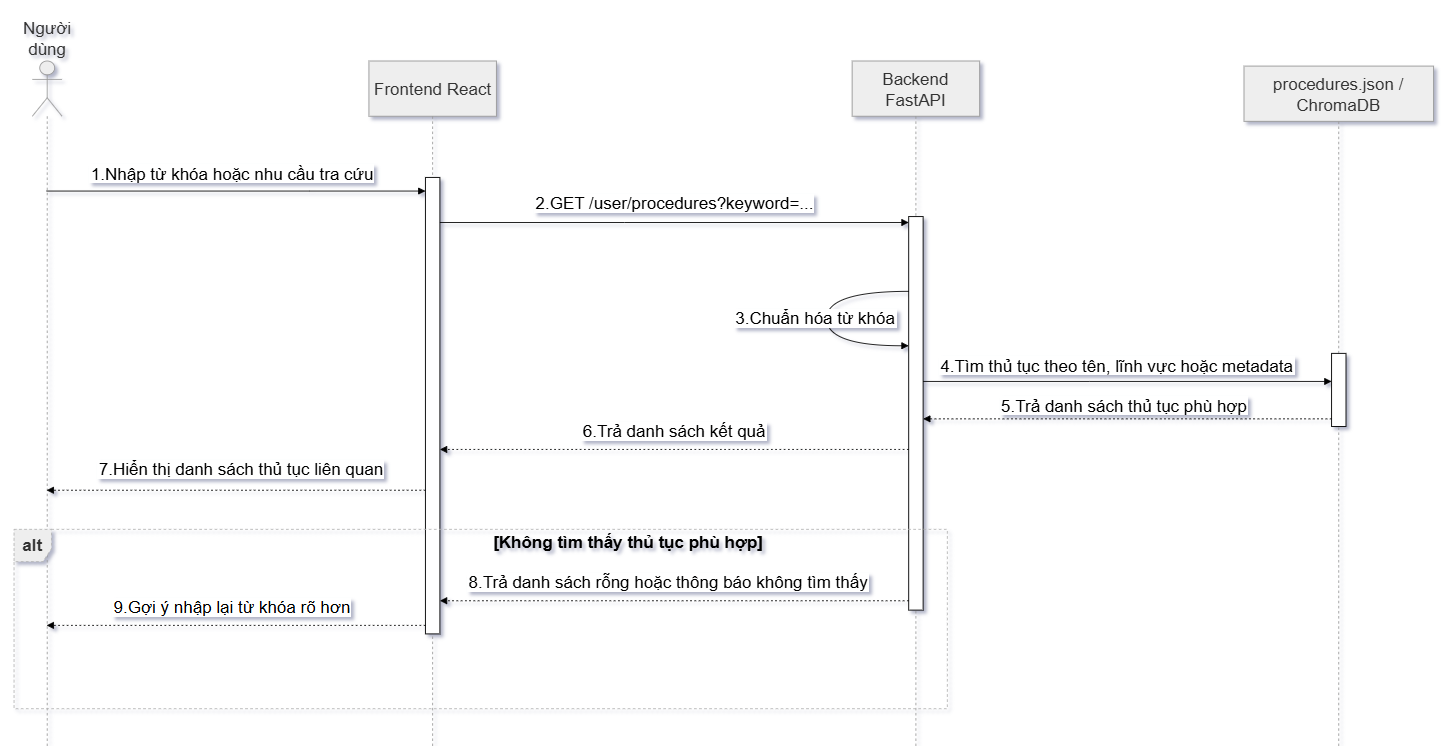
\includegraphics[width=0.92\textwidth]{tai_nguyen/media/image13.png}
\caption{Sơ đồ tuần tự luồng tra cứu TTHC}
\label{fig:3-7}
\end{figure}

\begin{figure}[H]
\centering
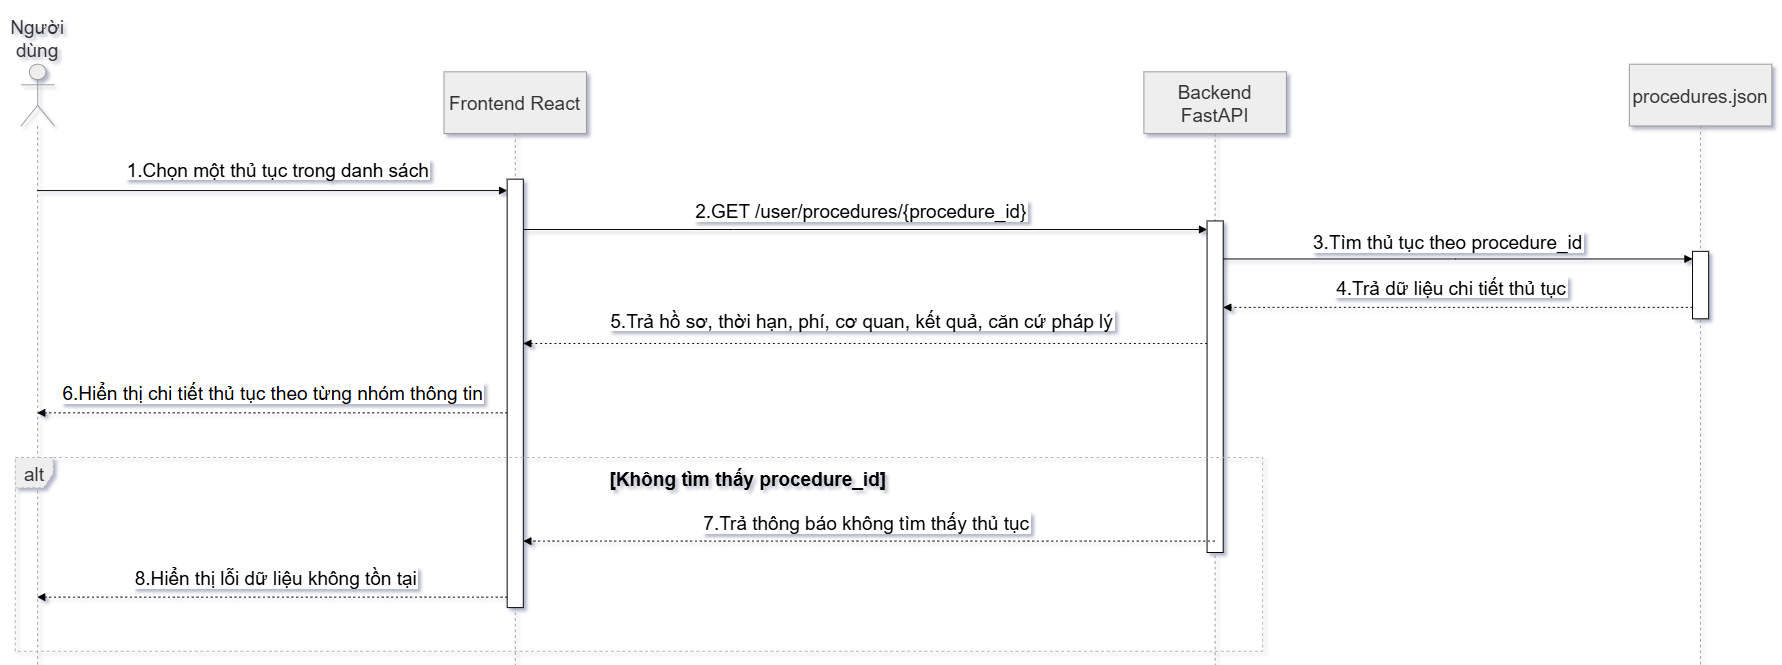
\includegraphics[width=0.92\textwidth]{tai_nguyen/media/image14.png}
\caption{Sơ đồ tuần tự luồng xem chi tiết thông tin thủ tục}
\label{fig:3-8}
\end{figure}

\begin{enumerate}
\def\labelenumi{\arabic{enumi}.}
\setcounter{enumi}{1}
\item
  \textbf{Thiết kế API hỏi đáp chatbot RAG}
\end{enumerate}

API /user/chat là luồng quan trọng nhất vì kết nối trực tiếp giao diện
hội thoại với pipeline RAG. Với thiết kế đề xuất, frontend gửi câu hỏi
và session\_id trong body JSON. Backend xác thực Firebase ID Token, lấy
lịch sử hội thoại gần nhất, gọi ask\_rag để tạo câu trả lời, sau đó lưu
tin nhắn vào Firestore. Response nên mở rộng thêm trường sources để hỗ
trợ trích dẫn nguồn trong tương lai.

\begin{figure}[H]
\centering
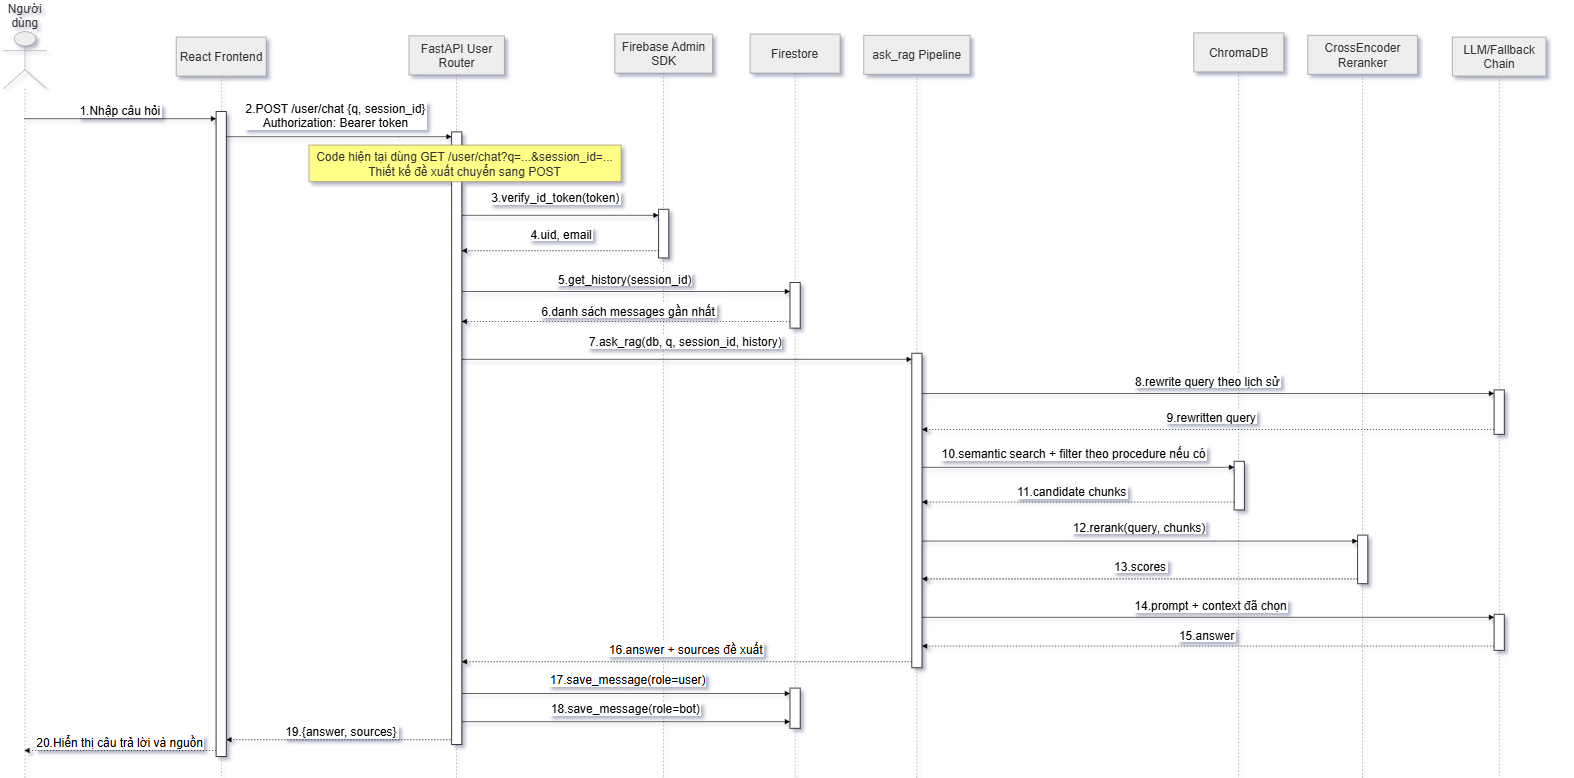
\includegraphics[width=0.92\textwidth]{tai_nguyen/media/image15.png}
\caption{Sơ đồ tuần tự xử lý API /user/chat}
\label{fig:3-9}
\end{figure}

\begin{enumerate}
\def\labelenumi{\arabic{enumi}.}
\setcounter{enumi}{2}
\item
  \textbf{Thiết kế API quản lý tài liệu và đồng bộ VectorDB}
\end{enumerate}

Nhóm API quản trị được bảo vệ bằng quyền admin ở backend. API
/admin/documents phục vụ xem, thêm, sửa, xóa dữ liệu thủ tục trong
procedures.json. Sau khi dữ liệu thay đổi, admin cần gọi
/admin/reload-vectordb để hệ thống đọc lại dữ liệu, tạo semantic chunks,
backup ChromaDB cũ và build lại vector database mới. Đây là luồng quan
trọng để kho tri thức của chatbot luôn đồng bộ với dữ liệu nguồn.

\begin{figure}[H]
\centering
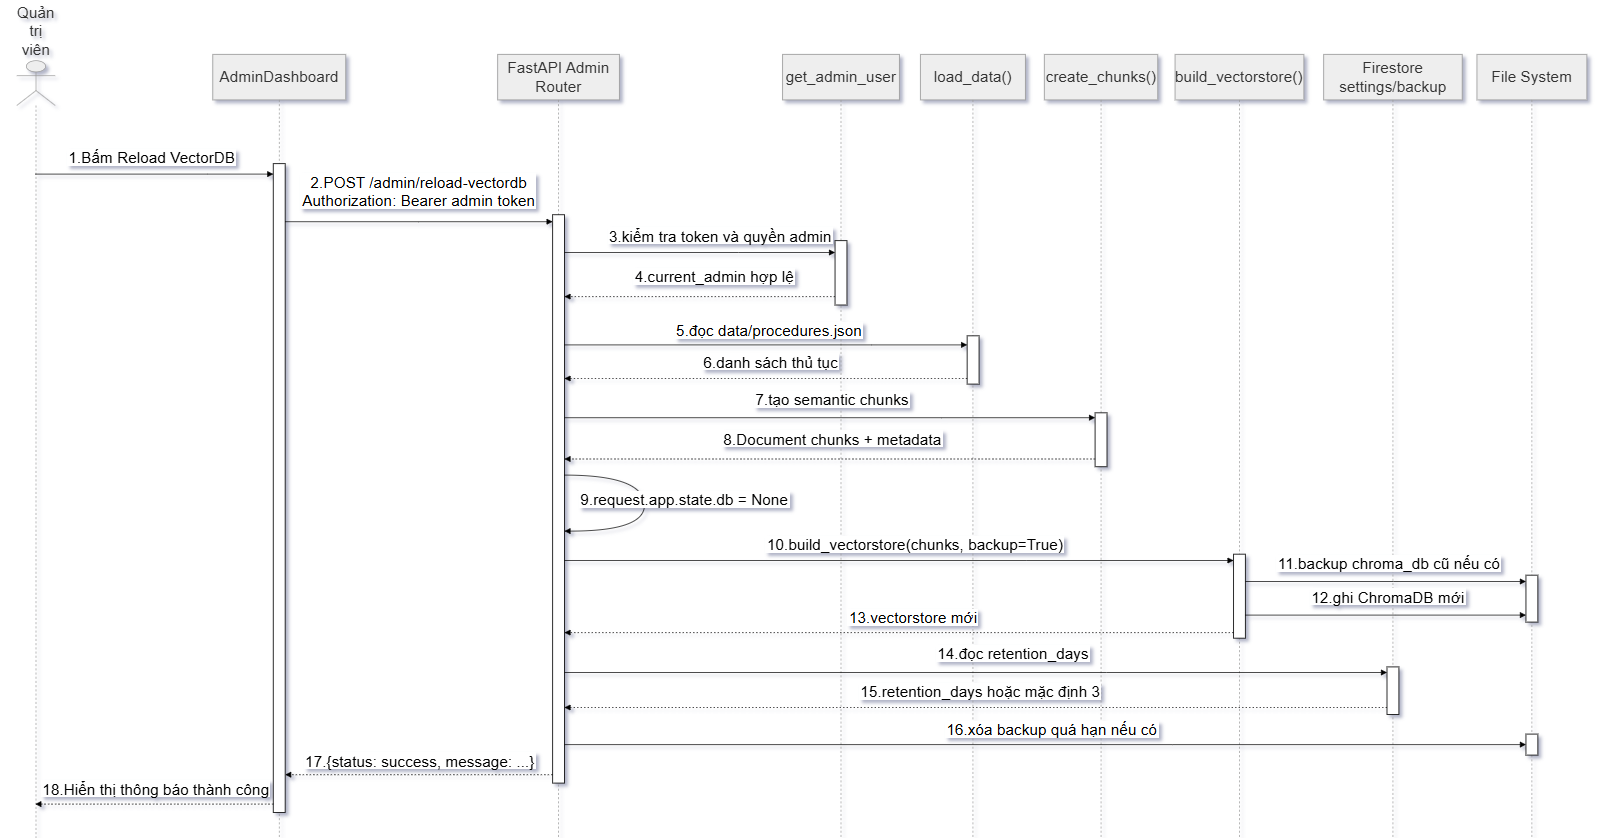
\includegraphics[width=0.92\textwidth]{tai_nguyen/media/image16.png}
\caption{Sơ đồ tuần tự đồng bộ VectorDB}
\label{fig:3-10}
\end{figure}

Như vậy, phần thiết kế API cần phân biệt rõ ba mức: API đã có trong mã
nguồn hiện tại, API nên chuyển đổi để đúng REST hơn và API đề xuất để
hoàn thiện Use Case tra cứu/xem chi tiết thủ tục. Cách trình bày này
giúp báo cáo vừa trung thực với code đã triển khai, vừa thể hiện được
hướng hoàn thiện hợp lý cho hệ thống.

\section{Thiết kế giao diện người dùng và
quản
trị}

Giao diện người dùng lấy khung hội thoại làm trung tâm. Người dân nhìn
thấy danh sách tin nhắn, ô nhập câu hỏi, câu hỏi gợi ý và sidebar lịch
sử. Khi câu trả lời dài, hệ thống ưu tiên xuống dòng và gạch đầu dòng để
người dùng dễ đọc trên điện thoại. Giao diện quản trị được tổ chức theo
tab để tách các nhóm chức năng: thống kê, lịch sử, tài liệu, backup và
quản lý admin.

Các component React phản ánh đúng trách nhiệm giao diện. App điều phối
trạng thái đăng nhập và phân quyền; LoginPage xử lý đăng nhập, đăng ký
và OTP; ChatBox điều phối hội thoại; Sidebar hiển thị session; InputBox
nhập câu hỏi; Message hiển thị tin nhắn; AdminDashboard phục vụ thao tác
quản trị. Cách chia component này giúp giao diện dễ bảo trì và dễ mở
rộng.

\begin{figure}[H]
\centering
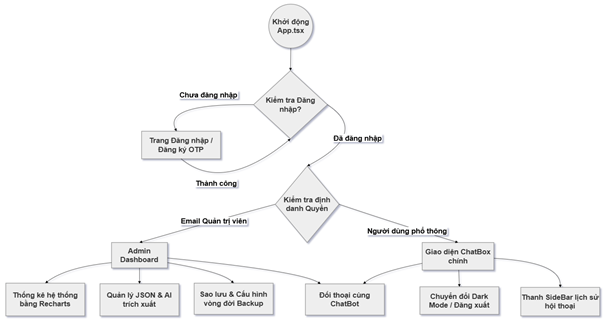
\includegraphics[width=0.92\textwidth]{tai_nguyen/media/image17.png}
\caption{Sitemap giao diện người dùng và quản trị viên thiết kế bảo mật và phân quyền}
\label{fig:3-11}
\end{figure}

\begin{figure}[H]
\centering
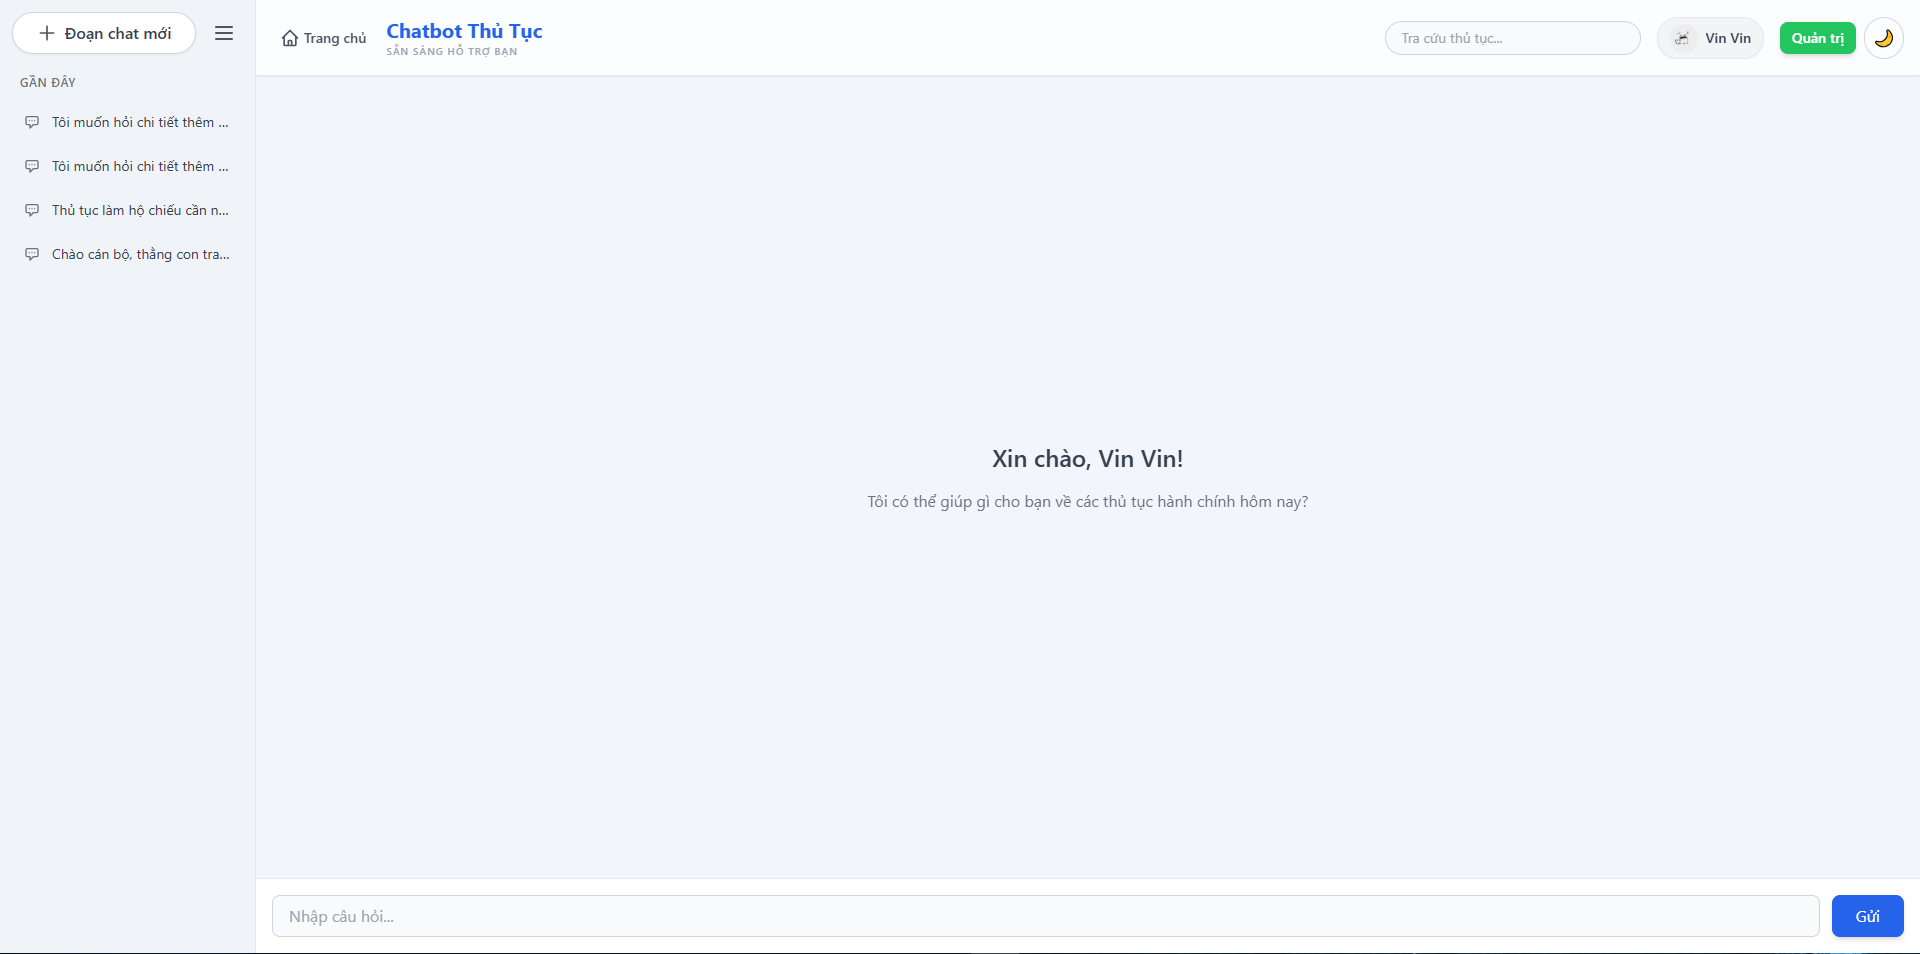
\includegraphics[width=0.92\textwidth]{tai_nguyen/media/image18.png}
\caption{Giao diện hỏi đáp TTHC bằng chatbot}
\label{fig:3-12}
\end{figure}

\begin{figure}[H]
\centering
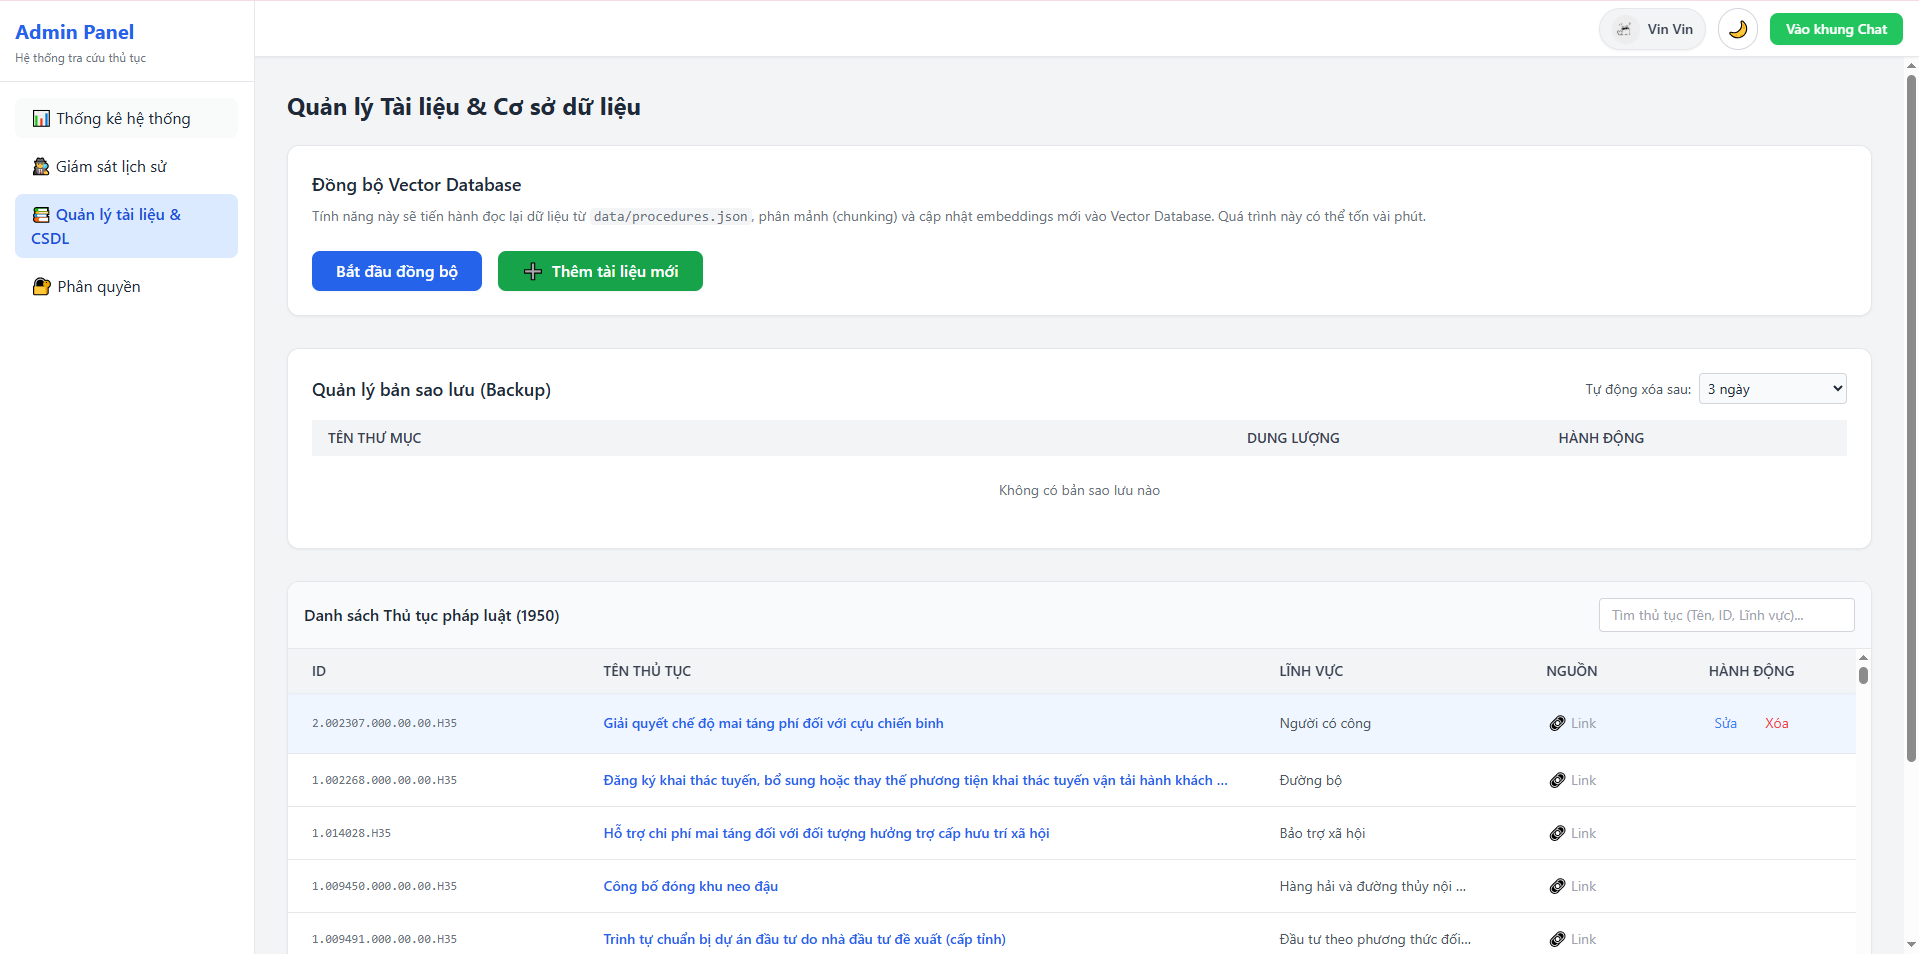
\includegraphics[width=0.92\textwidth]{tai_nguyen/media/image19.png}
\caption{Giao diện quản lý dữ liệu TTHC}
\label{fig:3-13}
\end{figure}

Bảo mật được kiểm soát chủ yếu ở backend. Frontend lấy Firebase ID Token
sau khi đăng nhập và gửi trong header Authorization. Backend dùng
Firebase Admin SDK để xác minh token. Với các endpoint /admin, backend
tiếp tục kiểm tra email trong danh sách admin hoặc custom claim thông
qua dependency get\_admin\_user. Cách làm này tránh tình trạng người
dùng chỉ cần sửa giao diện là truy cập được chức năng quản trị.

Dữ liệu nhạy cảm như serviceAccountKey, API key, sender password và
token không được đưa vào frontend. Các giá trị này cần đặt trong .env
hoặc secret của môi trường triển khai. Với ChromaDB, trước khi reload dữ
liệu cần backup thư mục cũ; sau khi build lại, hệ thống có thể dọn
backup quá hạn theo retention\_days để tránh tăng dung lượng không kiểm
soát.

Bảo mật RAG cũng được thiết kế ở tầng prompt. Mô hình chỉ được trả lời
theo context đã truy xuất; nếu dữ liệu không có, chatbot phải từ chối
trả lời thay vì suy đoán. Đây vừa là yêu cầu kỹ thuật, vừa là yêu cầu
nghiệp vụ trong hệ thống hành chính công.

\section{Thiết kế triển khai và cấu trúc mã
nguồn}

Hệ thống được triển khai theo kiến trúc web tách lớp. Người dùng thao
tác trên trình duyệt hoặc thiết bị di động thông qua giao diện React.
Backend FastAPI tiếp nhận request, xác thực người dùng, điều phối
pipeline RAG, gọi mô hình AI và ghi dữ liệu vận hành. Firebase
Authentication và Firestore phục vụ xác thực, lưu session, tin nhắn, OTP
và cấu hình quản trị. ChromaDB lưu vector embedding cùng metadata của
các đoạn dữ liệu TTHC.

\begin{figure}[H]
\centering
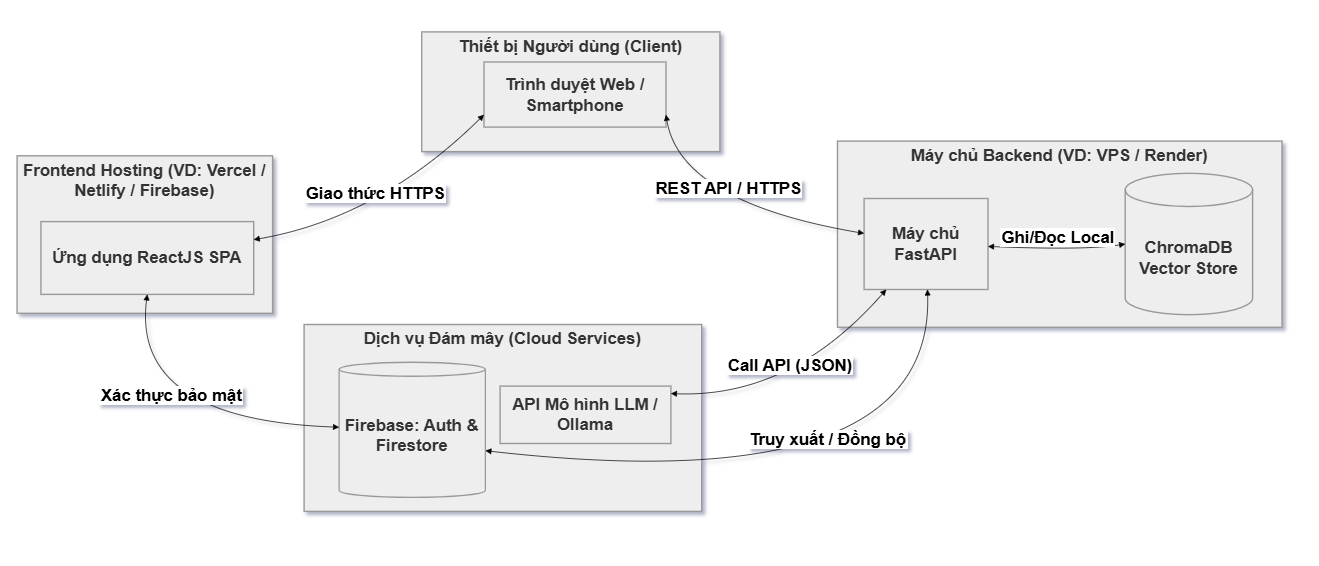
\includegraphics[width=0.92\textwidth]{tai_nguyen/media/image20.png}
\caption{Biểu đồ triển khai hệ thống (Deployment Diagram)}
\label{fig:3-14}
\end{figure}

Trong phạm vi thử nghiệm của đồ án, backend được khởi chạy bằng Uvicorn
trên cổng 8000. Khi cần truy cập từ môi trường bên ngoài hoặc demo trên
thiết bị khác, backend được mở ra Internet thông qua tunnel ngrok.
Frontend chạy bằng Vite và kết nối tới API URL tương ứng với backend
đang hoạt động.

\begin{longtable}[]{|
  >{\raggedright\arraybackslash}p{(\columnwidth - 4\tabcolsep) * \real{0.1514}}|
  >{\raggedright\arraybackslash}p{(\columnwidth - 4\tabcolsep) * \real{0.2659}}|
  >{\raggedright\arraybackslash}p{(\columnwidth - 4\tabcolsep) * \real{0.5827}}|}
\caption{Môi trường và thành phần triển khai}\\
\hline
\begin{minipage}[b]{\linewidth}\raggedright
\textbf{Thành phần}
\end{minipage} & \begin{minipage}[b]{\linewidth}\raggedright
\textbf{Công nghệ/công cụ}
\end{minipage} & \begin{minipage}[b]{\linewidth}\raggedright
\textbf{Vai trò}
\end{minipage} \\
\hline
\endfirsthead
\continuedcaption{Môi trường và thành phần triển khai}
\hline
\begin{minipage}[b]{\linewidth}\raggedright
\textbf{Thành phần}
\end{minipage} & \begin{minipage}[b]{\linewidth}\raggedright
\textbf{Công nghệ/công cụ}
\end{minipage} & \begin{minipage}[b]{\linewidth}\raggedright
\textbf{Vai trò}
\end{minipage} \\
\hline
\endhead
\hline
\endlastfoot
Backend & Python, FastAPI, Uvicorn & Cung cấp API, xác thực token, xử lý
RAG và quản trị dữ liệu. \\
\hline
Frontend & React, TypeScript, Vite & Xây dựng giao diện chatbot, đăng
nhập, lịch sử và dashboard quản trị. \\
\hline
Giao diện & Tailwind CSS, Recharts & Thiết kế responsive, dark mode và
biểu đồ thống kê. \\
\hline
AI/RAG & Ollama/Qwen, Gemini/OpenRouter, CrossEncoder & Rewrite câu hỏi,
truy xuất, rerank, sinh phản hồi và fallback. \\
\hline
Vector DB & ChromaDB & Lưu embedding và metadata của từng chunk thủ
tục. \\
\hline
Dữ liệu cloud & Firebase Authentication, Firestore & Xác thực, lưu lịch
sử chat, OTP, settings và danh sách admin. \\
\hline
\end{longtable}

\begin{longtable}[]{|
  >{\raggedright\arraybackslash}p{(\columnwidth - 4\tabcolsep) * \real{0.1949}}|
  >{\raggedright\arraybackslash}p{(\columnwidth - 4\tabcolsep) * \real{0.2773}}|
  >{\raggedright\arraybackslash}p{(\columnwidth - 4\tabcolsep) * \real{0.5278}}|}
\caption{Nhóm mã nguồn backend và vai trò}\\
\hline
\begin{minipage}[b]{\linewidth}\raggedright
\textbf{Nhóm}
\end{minipage} & \begin{minipage}[b]{\linewidth}\raggedright
\textbf{File tiêu biểu}
\end{minipage} & \begin{minipage}[b]{\linewidth}\raggedright
\textbf{Vai trò}
\end{minipage} \\
\hline
\endfirsthead
\continuedcaption{Nhóm mã nguồn backend và vai trò}
\hline
\begin{minipage}[b]{\linewidth}\raggedright
\textbf{Nhóm}
\end{minipage} & \begin{minipage}[b]{\linewidth}\raggedright
\textbf{File tiêu biểu}
\end{minipage} & \begin{minipage}[b]{\linewidth}\raggedright
\textbf{Vai trò}
\end{minipage} \\
\hline
\endhead
\hline
\endlastfoot
Khởi động ứng dụng & main.py & Khởi tạo FastAPI, Firebase, CORS, router
và load/build ChromaDB. \\
\hline
Xử lý dữ liệu & loader.py, chunker.py, vectorstore.py & Đọc
procedures.json, chia chunk và lưu embedding vào ChromaDB. \\
\hline
Hỏi đáp RAG & pipeline.py, normalizer.py, intent.py & Chuẩn hóa câu hỏi,
nhận diện intent, retrieval, rerank, prompt và gọi LLM. \\
\hline
Bộ nhớ hội thoại & memory.py & Đọc và ghi lịch sử chat theo session
trong Firestore. \\
\hline
Router API & auth.py, user.py, admin.py & Xác thực, chat người dùng,
quản trị dữ liệu, backup và reload VectorDB. \\
\hline
\end{longtable}

Bảng 3.7 chỉ trình bày các nhóm mã nguồn chính để người đọc nắm được cấu
trúc triển khai. Cấu trúc thư mục backend và frontend được trình bày cụ
thể tại Phụ lục A.

\begin{figure}[H]
\centering
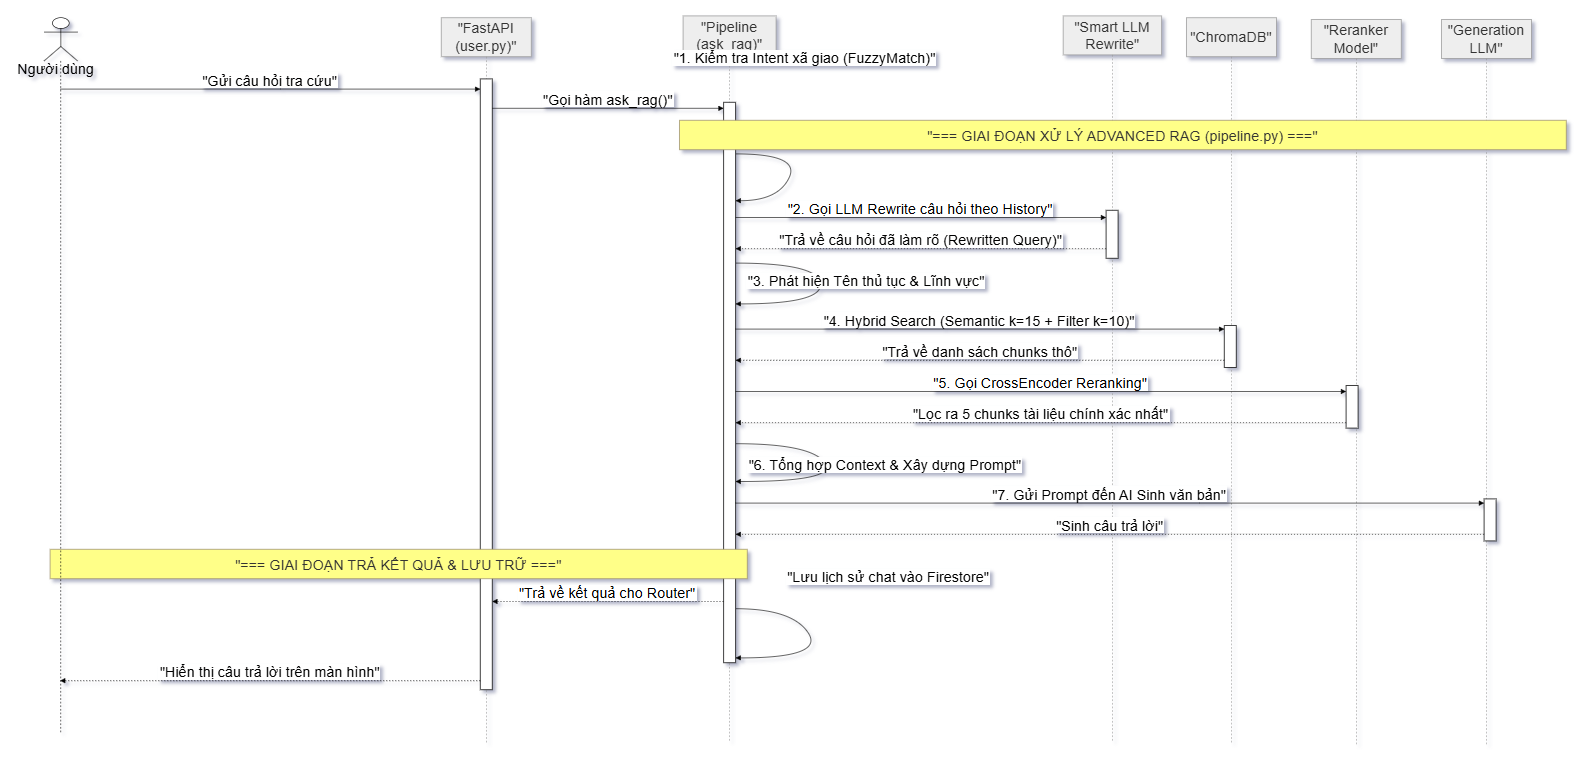
\includegraphics[width=0.92\textwidth]{tai_nguyen/media/image21.png}
\caption{Sơ đồ tuần tự xử lý Pipeline Advanced RAG chi tiết}
\label{fig:3-15}
\end{figure}

Khi backend khởi động, hệ thống ưu tiên nạp ChromaDB đã tồn tại. Nếu
chưa có vector database, backend đọc procedures.json, tạo semantic
chunks, sinh embedding và lưu vào ChromaDB. Trong quá trình hỏi đáp,
pipeline xử lý intent, viết lại câu hỏi theo lịch sử, chuẩn hóa synonym,
truy xuất vector, rerank bằng CrossEncoder và gọi LLM để sinh câu trả
lời dựa trên context.

\begin{figure}[H]
\centering
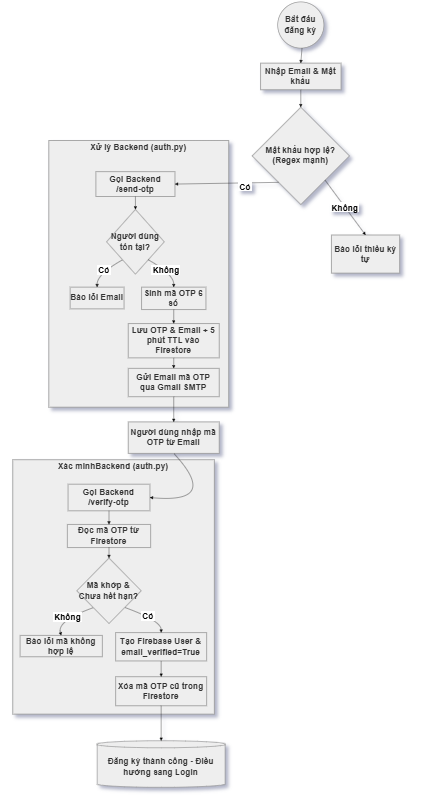
\includegraphics[height=0.74\textheight,keepaspectratio]{tai_nguyen/media/image22.png}
\caption{Lưu đồ thuật toán đăng ký và xác thực OTP}
\label{fig:3-16}
\end{figure}

\begin{figure}[H]
\centering
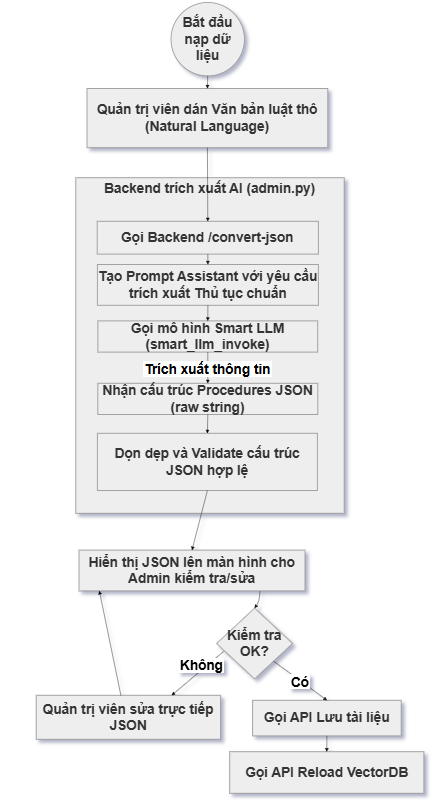
\includegraphics[height=0.74\textheight,keepaspectratio]{tai_nguyen/media/image23.png}
\caption{Lưu đồ trích xuất JSON bằng AI cho quản trị viên}
\label{fig:3-17}
\end{figure}

\begin{figure}[H]
\centering
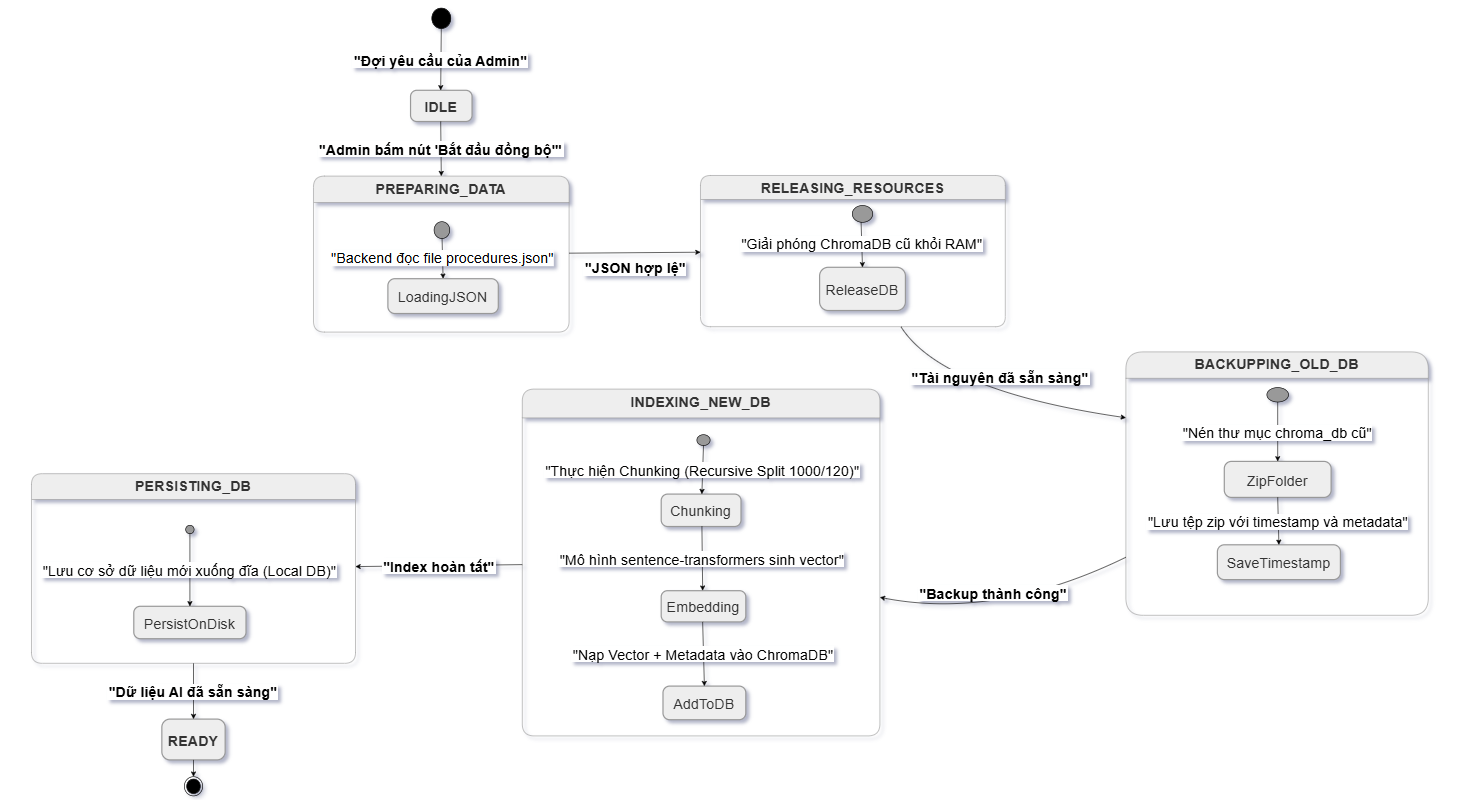
\includegraphics[width=0.92\textwidth]{tai_nguyen/media/image24.png}
\caption{Biểu đồ trạng thái đồng bộ và sao lưu VectorDB}
\label{fig:3-18}
\end{figure}
